\documentclass[twoside]{book}

% Packages required by doxygen
\usepackage{fixltx2e}
\usepackage{calc}
\usepackage{doxygen}
\usepackage[export]{adjustbox} % also loads graphicx
\usepackage{graphicx}
\usepackage[utf8]{inputenc}
\usepackage{makeidx}
\usepackage{multicol}
\usepackage{multirow}
\PassOptionsToPackage{warn}{textcomp}
\usepackage{textcomp}
\usepackage[nointegrals]{wasysym}
\usepackage[table]{xcolor}

% Font selection
\usepackage[T1]{fontenc}
\usepackage[scaled=.90]{helvet}
\usepackage{courier}
\usepackage{amssymb}
\usepackage{sectsty}
\renewcommand{\familydefault}{\sfdefault}
\allsectionsfont{%
  \fontseries{bc}\selectfont%
  \color{darkgray}%
}
\renewcommand{\DoxyLabelFont}{%
  \fontseries{bc}\selectfont%
  \color{darkgray}%
}
\newcommand{\+}{\discretionary{\mbox{\scriptsize$\hookleftarrow$}}{}{}}

% Page & text layout
\usepackage{geometry}
\geometry{%
  a4paper,%
  top=2.5cm,%
  bottom=2.5cm,%
  left=2.5cm,%
  right=2.5cm%
}
\tolerance=750
\hfuzz=15pt
\hbadness=750
\setlength{\emergencystretch}{15pt}
\setlength{\parindent}{0cm}
\setlength{\parskip}{0.2cm}
\makeatletter
\renewcommand{\paragraph}{%
  \@startsection{paragraph}{4}{0ex}{-1.0ex}{1.0ex}{%
    \normalfont\normalsize\bfseries\SS@parafont%
  }%
}
\renewcommand{\subparagraph}{%
  \@startsection{subparagraph}{5}{0ex}{-1.0ex}{1.0ex}{%
    \normalfont\normalsize\bfseries\SS@subparafont%
  }%
}
\makeatother

% Headers & footers
\usepackage{fancyhdr}
\pagestyle{fancyplain}
\fancyhead[LE]{\fancyplain{}{\bfseries\thepage}}
\fancyhead[CE]{\fancyplain{}{}}
\fancyhead[RE]{\fancyplain{}{\bfseries\leftmark}}
\fancyhead[LO]{\fancyplain{}{\bfseries\rightmark}}
\fancyhead[CO]{\fancyplain{}{}}
\fancyhead[RO]{\fancyplain{}{\bfseries\thepage}}
\fancyfoot[LE]{\fancyplain{}{}}
\fancyfoot[CE]{\fancyplain{}{}}
\fancyfoot[RE]{\fancyplain{}{\bfseries\scriptsize Generated on Sat Feb 18 2017 19\+:25\+:44 for My Project by Doxygen }}
\fancyfoot[LO]{\fancyplain{}{\bfseries\scriptsize Generated on Sat Feb 18 2017 19\+:25\+:44 for My Project by Doxygen }}
\fancyfoot[CO]{\fancyplain{}{}}
\fancyfoot[RO]{\fancyplain{}{}}
\renewcommand{\footrulewidth}{0.4pt}
\renewcommand{\chaptermark}[1]{%
  \markboth{#1}{}%
}
\renewcommand{\sectionmark}[1]{%
  \markright{\thesection\ #1}%
}

% Indices & bibliography
\usepackage{natbib}
\usepackage[titles]{tocloft}
\setcounter{tocdepth}{3}
\setcounter{secnumdepth}{5}
\makeindex

% Hyperlinks (required, but should be loaded last)
\usepackage{ifpdf}
\ifpdf
  \usepackage[pdftex,pagebackref=true]{hyperref}
\else
  \usepackage[ps2pdf,pagebackref=true]{hyperref}
\fi
\hypersetup{%
  colorlinks=true,%
  linkcolor=blue,%
  citecolor=blue,%
  unicode%
}

% Custom commands
\newcommand{\clearemptydoublepage}{%
  \newpage{\pagestyle{empty}\cleardoublepage}%
}


%===== C O N T E N T S =====

\begin{document}

% Titlepage & ToC
\hypersetup{pageanchor=false,
             bookmarks=true,
             bookmarksnumbered=true,
             pdfencoding=unicode
            }
\pagenumbering{roman}
\begin{titlepage}
\vspace*{7cm}
\begin{center}%
{\Large My Project }\\
\vspace*{1cm}
{\large Generated by Doxygen 1.8.9.1}\\
\vspace*{0.5cm}
{\small Sat Feb 18 2017 19:25:44}\\
\end{center}
\end{titlepage}
\clearemptydoublepage
\tableofcontents
\clearemptydoublepage
\pagenumbering{arabic}
\hypersetup{pageanchor=true}

%--- Begin generated contents ---
\chapter{Hierarchical Index}
\section{Class Hierarchy}
This inheritance list is sorted roughly, but not completely, alphabetically\+:\begin{DoxyCompactList}
\item J\+Frame\begin{DoxyCompactList}
\item \contentsline{section}{Main\+Frame\+Part1}{\pageref{classMainFramePart1}}{}
\item \contentsline{section}{Main\+Frame\+Part2}{\pageref{classMainFramePart2}}{}
\item \contentsline{section}{Remote\+Control}{\pageref{classRemoteControl}}{}
\end{DoxyCompactList}
\item \contentsline{section}{Remote\+Client}{\pageref{classRemoteClient}}{}
\end{DoxyCompactList}

\chapter{Class Index}
\section{Class List}
Here are the classes, structs, unions and interfaces with brief descriptions\+:\begin{DoxyCompactList}
\item\contentsline{section}{\hyperlink{structcppu_1_1TCPServer_1_1Callback}{cppu\+::\+T\+C\+P\+Server\+::\+Callback} \\*\hyperlink{structcppu_1_1TCPServer_1_1Callback}{Callback} interface }{\pageref{structcppu_1_1TCPServer_1_1Callback}}{}
\item\contentsline{section}{\hyperlink{structcppu_1_1TCPServer_1_1CallbackMethod}{cppu\+::\+T\+C\+P\+Server\+::\+Callback\+Method$<$ T $>$} }{\pageref{structcppu_1_1TCPServer_1_1CallbackMethod}}{}
\item\contentsline{section}{\hyperlink{classData}{Data} \\*\hyperlink{classData}{Data} class. This is the class which is used to keep tracks of all the multimediaobjects and groups created. \hyperlink{classData}{Data} is stored using std\+::map, using names as keys. We use smart pointers everywhere for a better memory usage }{\pageref{classData}}{}
\item\contentsline{section}{\hyperlink{classFilm}{Film} \\*\hyperlink{classFilm}{Film} class, extends the video class. Using pointers for learning purpose }{\pageref{classFilm}}{}
\item\contentsline{section}{\hyperlink{classGroup}{Group} \\*\hyperlink{classGroup}{Group} class extends the std\+::list class. We store shared\+\_\+ptr of multimedia objects to prevent any memory leak }{\pageref{classGroup}}{}
\item\contentsline{section}{\hyperlink{structcppu_1_1InputBuffer}{cppu\+::\+Input\+Buffer} }{\pageref{structcppu_1_1InputBuffer}}{}
\item\contentsline{section}{\hyperlink{classMultimediaObject}{Multimedia\+Object} \\*Abstract class for a multimedia object }{\pageref{classMultimediaObject}}{}
\item\contentsline{section}{\hyperlink{classPicture}{Picture} \\*\hyperlink{classPicture}{Picture} class, extends the abstract class \hyperlink{classMultimediaObject}{Multimedia\+Object} }{\pageref{classPicture}}{}
\item\contentsline{section}{\hyperlink{classcppu_1_1ServerSocket}{cppu\+::\+Server\+Socket} \\*T\+C\+P/\+I\+P server socket. This class implements a T\+C\+P/\+I\+P socket that waits for requests to come in over the network. A\+F\+\_\+\+I\+N\+E\+T connections following the I\+Pv4 Internet protocol are supported }{\pageref{classcppu_1_1ServerSocket}}{}
\item\contentsline{section}{\hyperlink{classcppu_1_1Socket}{cppu\+::\+Socket} \\*T\+C\+P/\+I\+P or U\+D\+P/\+Datagram socket. This class encapsulates a T\+C\+P/\+I\+P or U\+D\+P/\+Datagram socket. A\+F\+\_\+\+I\+N\+E\+T connections following the I\+Pv4 Internet protocol are supported }{\pageref{classcppu_1_1Socket}}{}
\item\contentsline{section}{\hyperlink{classcppu_1_1SocketBuffer}{cppu\+::\+Socket\+Buffer} \\*Preserves record boundaries when exchanging data between connected T\+C\+P/\+I\+P sockets. This class ensures that one call to \hyperlink{classcppu_1_1SocketBuffer_a92ae0351aaee8719d34e8c4618495d59}{write\+Line()} corresponds to one and exactly one call to \hyperlink{classcppu_1_1SocketBuffer_a222769d3776b9cbd3a727ee1f0e60358}{read\+Line()} on the other side. This differs from the behavior of \hyperlink{classcppu_1_1Socket_aeac77f859159715e2d63a5a0dc118788}{Socket\+::send()} and \hyperlink{classcppu_1_1Socket_a37c382af52cc02f92c0e19a0c6e0e04f}{Socket\+::receive()} because T\+C\+P/\+I\+P connected sockets do not preserve record boundaries. \hyperlink{classcppu_1_1SocketBuffer_a92ae0351aaee8719d34e8c4618495d59}{write\+Line()} and \hyperlink{classcppu_1_1SocketBuffer_a222769d3776b9cbd3a727ee1f0e60358}{read\+Line()} solve this problem by automatically adding and searching for a separator between successive lines }{\pageref{classcppu_1_1SocketBuffer}}{}
\item\contentsline{section}{\hyperlink{classcppu_1_1TCPConnection}{cppu\+::\+T\+C\+P\+Connection} \\*Connection with a given client. Each \hyperlink{classcppu_1_1TCPConnection}{T\+C\+P\+Connection} uses a different thread }{\pageref{classcppu_1_1TCPConnection}}{}
\item\contentsline{section}{\hyperlink{classcppu_1_1TCPLock}{cppu\+::\+T\+C\+P\+Lock} \\*Locks the server in read mode or in write mode. Must be created {\itshape in the stack} by the callback method }{\pageref{classcppu_1_1TCPLock}}{}
\item\contentsline{section}{\hyperlink{classcppu_1_1TCPServer}{cppu\+::\+T\+C\+P\+Server} \\*T\+C\+P/\+I\+P I\+Pv4 server. The server supports T\+C\+P/\+I\+P A\+F\+\_\+\+I\+N\+E\+T connections (following the I\+Pv4 Internet protocol) with multiple clients. One thread is used per client }{\pageref{classcppu_1_1TCPServer}}{}
\item\contentsline{section}{\hyperlink{classVideo}{Video} \\*\hyperlink{classVideo}{Video} class, extends the abstract class \hyperlink{classMultimediaObject}{Multimedia\+Object} }{\pageref{classVideo}}{}
\end{DoxyCompactList}

\chapter{Class Documentation}
\hypertarget{classMainFramePart1}{}\section{Main\+Frame\+Part1 Class Reference}
\label{classMainFramePart1}\index{Main\+Frame\+Part1@{Main\+Frame\+Part1}}


Inheritance diagram for Main\+Frame\+Part1\+:
\nopagebreak
\begin{figure}[H]
\begin{center}
\leavevmode
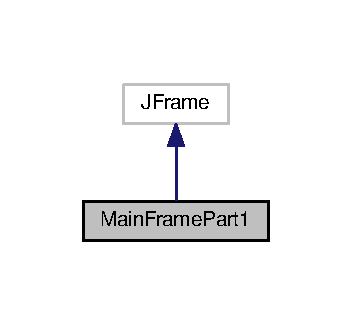
\includegraphics[width=169pt]{classMainFramePart1__inherit__graph}
\end{center}
\end{figure}


Collaboration diagram for Main\+Frame\+Part1\+:
\nopagebreak
\begin{figure}[H]
\begin{center}
\leavevmode
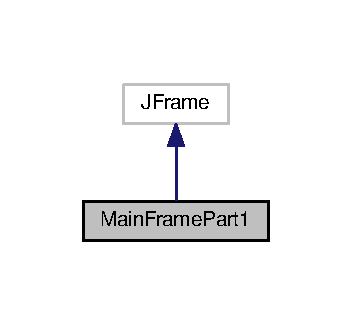
\includegraphics[width=169pt]{classMainFramePart1__coll__graph}
\end{center}
\end{figure}
\subsection*{Classes}
\begin{DoxyCompactItemize}
\item 
class {\bfseries Bonjour\+Listener}
\item 
class {\bfseries Exit\+Listener}
\item 
class {\bfseries Hello\+Listener}
\end{DoxyCompactItemize}
\subsection*{Static Public Member Functions}
\begin{DoxyCompactItemize}
\item 
\hypertarget{classMainFramePart1_a7facdd552ebf47dcc8b8372ea6875c12}{}static void {\bfseries main} (String argv\mbox{[}$\,$\mbox{]})\label{classMainFramePart1_a7facdd552ebf47dcc8b8372ea6875c12}

\end{DoxyCompactItemize}


The documentation for this class was generated from the following file\+:\begin{DoxyCompactItemize}
\item 
Main\+Frame\+Part1.\+java\end{DoxyCompactItemize}

\hypertarget{classMainFramePart2}{}\section{Main\+Frame\+Part2 Class Reference}
\label{classMainFramePart2}\index{Main\+Frame\+Part2@{Main\+Frame\+Part2}}


Inheritance diagram for Main\+Frame\+Part2\+:
\nopagebreak
\begin{figure}[H]
\begin{center}
\leavevmode
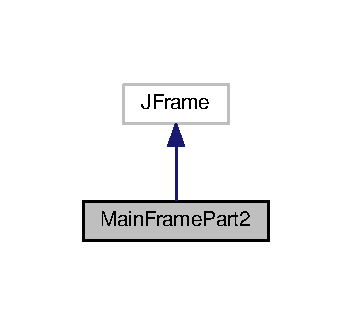
\includegraphics[width=169pt]{classMainFramePart2__inherit__graph}
\end{center}
\end{figure}


Collaboration diagram for Main\+Frame\+Part2\+:
\nopagebreak
\begin{figure}[H]
\begin{center}
\leavevmode
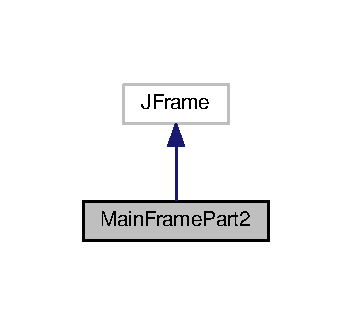
\includegraphics[width=169pt]{classMainFramePart2__coll__graph}
\end{center}
\end{figure}
\subsection*{Classes}
\begin{DoxyCompactItemize}
\item 
class {\bfseries Bonjour\+Action}
\item 
class {\bfseries Exit\+Action}
\item 
class {\bfseries Hello\+Action}
\end{DoxyCompactItemize}
\subsection*{Static Public Member Functions}
\begin{DoxyCompactItemize}
\item 
\hypertarget{classMainFramePart2_a80b537b240ec1e16ea6b3c9ce4c9d544}{}static void {\bfseries main} (String argv\mbox{[}$\,$\mbox{]})\label{classMainFramePart2_a80b537b240ec1e16ea6b3c9ce4c9d544}

\end{DoxyCompactItemize}


The documentation for this class was generated from the following file\+:\begin{DoxyCompactItemize}
\item 
Main\+Frame\+Part2.\+java\end{DoxyCompactItemize}

\hypertarget{classRemoteClient}{}\section{Remote\+Client Class Reference}
\label{classRemoteClient}\index{Remote\+Client@{Remote\+Client}}
\subsection*{Public Member Functions}
\begin{DoxyCompactItemize}
\item 
\hyperlink{classRemoteClient_a39280daa273d198244dd7084b1150313}{Remote\+Client} (String host, int port)  throws Unknown\+Host\+Exception, I\+O\+Exception 
\item 
String \hyperlink{classRemoteClient_ad14bdcb0ae285619ce231f8e6aad6b0b}{send} (String request)
\end{DoxyCompactItemize}


\subsection{Constructor \& Destructor Documentation}
\hypertarget{classRemoteClient_a39280daa273d198244dd7084b1150313}{}\index{Remote\+Client@{Remote\+Client}!Remote\+Client@{Remote\+Client}}
\index{Remote\+Client@{Remote\+Client}!Remote\+Client@{Remote\+Client}}
\subsubsection[{Remote\+Client}]{\setlength{\rightskip}{0pt plus 5cm}Remote\+Client.\+Remote\+Client (
\begin{DoxyParamCaption}
\item[{String}]{host, }
\item[{int}]{port}
\end{DoxyParamCaption}
) throws Unknown\+Host\+Exception, I\+O\+Exception\hspace{0.3cm}{\ttfamily [inline]}}\label{classRemoteClient_a39280daa273d198244dd7084b1150313}
Initialise la connexion. Renvoie une exception en cas d\textquotesingle{}erreur. 

\subsection{Member Function Documentation}
\hypertarget{classRemoteClient_ad14bdcb0ae285619ce231f8e6aad6b0b}{}\index{Remote\+Client@{Remote\+Client}!send@{send}}
\index{send@{send}!Remote\+Client@{Remote\+Client}}
\subsubsection[{send}]{\setlength{\rightskip}{0pt plus 5cm}String Remote\+Client.\+send (
\begin{DoxyParamCaption}
\item[{String}]{request}
\end{DoxyParamCaption}
)\hspace{0.3cm}{\ttfamily [inline]}}\label{classRemoteClient_ad14bdcb0ae285619ce231f8e6aad6b0b}
Envoie une requete au server et retourne sa reponse. Noter que la methode bloque si le serveur ne repond pas. 

The documentation for this class was generated from the following file\+:\begin{DoxyCompactItemize}
\item 
Remote\+Client.\+java\end{DoxyCompactItemize}

\hypertarget{classRemoteControl}{}\section{Remote\+Control Class Reference}
\label{classRemoteControl}\index{Remote\+Control@{Remote\+Control}}


Inheritance diagram for Remote\+Control\+:
\nopagebreak
\begin{figure}[H]
\begin{center}
\leavevmode
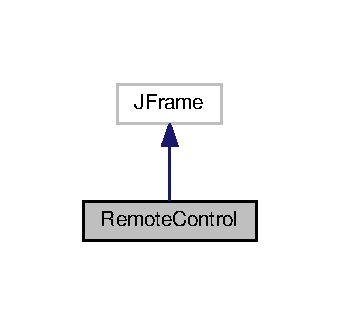
\includegraphics[width=163pt]{classRemoteControl__inherit__graph}
\end{center}
\end{figure}


Collaboration diagram for Remote\+Control\+:
\nopagebreak
\begin{figure}[H]
\begin{center}
\leavevmode
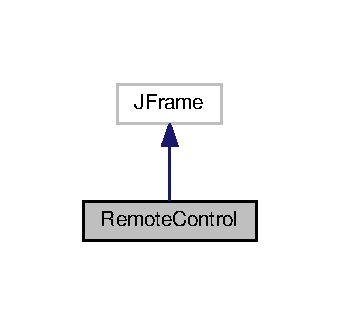
\includegraphics[width=163pt]{classRemoteControl__coll__graph}
\end{center}
\end{figure}
\subsection*{Classes}
\begin{DoxyCompactItemize}
\item 
class {\bfseries Exit\+Action}
\item 
class {\bfseries Send\+Request\+Action}
\end{DoxyCompactItemize}
\subsection*{Public Member Functions}
\begin{DoxyCompactItemize}
\item 
\hyperlink{classRemoteControl_adbe3adb1e50b865dd7b0937715b40332}{Remote\+Control} (\hyperlink{classRemoteClient}{Remote\+Client} client)
\item 
void \hyperlink{classRemoteControl_a0c45149dda61f4878eb839971324960c}{send\+Request} ()
\end{DoxyCompactItemize}
\subsection*{Static Public Member Functions}
\begin{DoxyCompactItemize}
\item 
static void \hyperlink{classRemoteControl_ac00de0c62936316ebf7dedc9ca08ea7b}{main} (String argv\mbox{[}$\,$\mbox{]})
\end{DoxyCompactItemize}


\subsection{Constructor \& Destructor Documentation}
\hypertarget{classRemoteControl_adbe3adb1e50b865dd7b0937715b40332}{}\index{Remote\+Control@{Remote\+Control}!Remote\+Control@{Remote\+Control}}
\index{Remote\+Control@{Remote\+Control}!Remote\+Control@{Remote\+Control}}
\subsubsection[{Remote\+Control}]{\setlength{\rightskip}{0pt plus 5cm}Remote\+Control.\+Remote\+Control (
\begin{DoxyParamCaption}
\item[{{\bf Remote\+Client}}]{client}
\end{DoxyParamCaption}
)\hspace{0.3cm}{\ttfamily [inline]}}\label{classRemoteControl_adbe3adb1e50b865dd7b0937715b40332}
The client

Behaviour of text\+Areas. request\+Text Area is where the user writes the request reponse\+Text\+Area is non editable \+: this is where we write answers from the server.

Here we add a listener to the request\+Area so tha pressing enter will send the message.

Creating labels.

Creating actions.

Creating the menu.

Creating the toolbar.

Putting the layout together.

Behaviour of the J\+Frame. 

\subsection{Member Function Documentation}
\hypertarget{classRemoteControl_ac00de0c62936316ebf7dedc9ca08ea7b}{}\index{Remote\+Control@{Remote\+Control}!main@{main}}
\index{main@{main}!Remote\+Control@{Remote\+Control}}
\subsubsection[{main}]{\setlength{\rightskip}{0pt plus 5cm}static void Remote\+Control.\+main (
\begin{DoxyParamCaption}
\item[{String}]{argv\mbox{[}$\,$\mbox{]}}
\end{DoxyParamCaption}
)\hspace{0.3cm}{\ttfamily [inline]}, {\ttfamily [static]}}\label{classRemoteControl_ac00de0c62936316ebf7dedc9ca08ea7b}
main function where we create the remote controle and the client. \hypertarget{classRemoteControl_a0c45149dda61f4878eb839971324960c}{}\index{Remote\+Control@{Remote\+Control}!send\+Request@{send\+Request}}
\index{send\+Request@{send\+Request}!Remote\+Control@{Remote\+Control}}
\subsubsection[{send\+Request}]{\setlength{\rightskip}{0pt plus 5cm}void Remote\+Control.\+send\+Request (
\begin{DoxyParamCaption}
{}
\end{DoxyParamCaption}
)\hspace{0.3cm}{\ttfamily [inline]}}\label{classRemoteControl_a0c45149dda61f4878eb839971324960c}
Sends the request in the request\+Text\+Area and displays the answer from the server in the response\+Text\+Area. 

The documentation for this class was generated from the following file\+:\begin{DoxyCompactItemize}
\item 
Remote\+Control.\+java\end{DoxyCompactItemize}

%--- End generated contents ---

% Index
\backmatter
\newpage
\phantomsection
\clearemptydoublepage
\addcontentsline{toc}{chapter}{Index}
\printindex

\end{document}
